A versão \texttt{q03a} (sequencial) possui o tempo mais curto de execução dos cálculos da célula da matriz resultante, com tempos na ordem de grandeza de $10^2 \ \text{ns}$  para os casos de teste fornecidos. Em seguida, a versão \texttt{q03b} (concorrente, limitado pela quantitade de processadores no sistema computacional) apresenta tempos na ordem de grandeza de $10^4$ à $10^6 \ \text{ns}$. Por fim, a versão \texttt{q03c} (concorrente, não limitado) apresenta tempos na mesma ordem de grandeza que a versão \texttt{q03b}, de $10^4$ à $10^6 \ \text{ns}$, porém, seus valores apresentados são, em média, $14\%$ maiores que a versão \texttt{q03b} quando o número total de células da matriz resultante é superior ao número total de processadores no sistema computacional. As figuras a seguir descrevem os resultados de três execuções de cada versão de código em cada o caso de teste fornecido pelo Makefile.

\begin{figure}[H]
	\begin{center}
		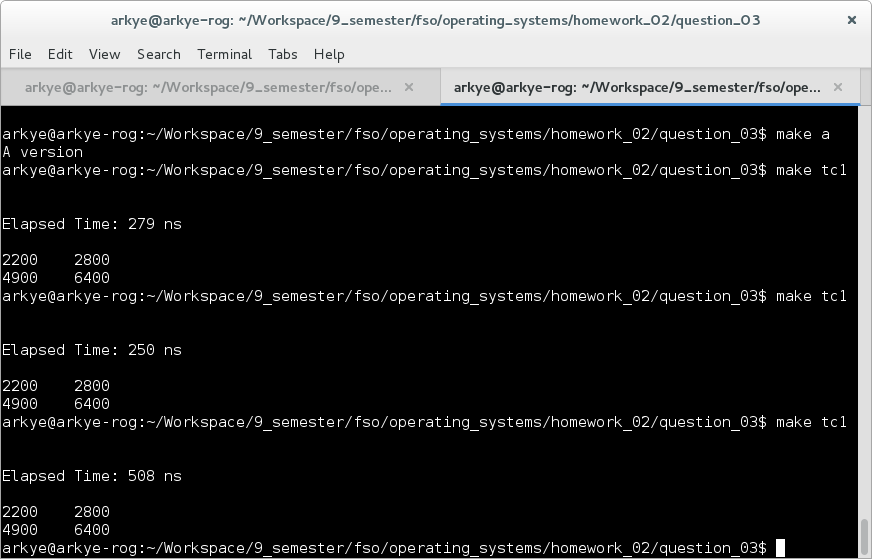
\includegraphics[scale=0.399]{a_tc1}
		\caption{Resultados da versão \texttt{q03a} com o caso de teste \texttt{tc1}.}
		\label{fig:a_tc1}
	\end{center}
\end{figure}

\begin{figure}[H]
	\begin{center}
		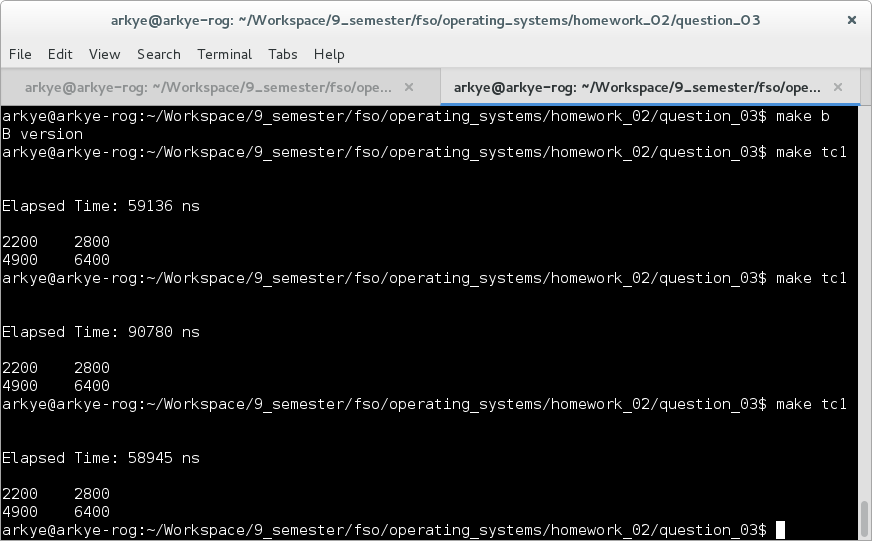
\includegraphics[scale=0.4]{b_tc1}
		\caption{Resultados da versão \texttt{q03b} com o caso de teste \texttt{tc1}.}
		\label{fig:b_tc1}
	\end{center}
\end{figure}

\begin{figure}[H]
	\begin{center}
		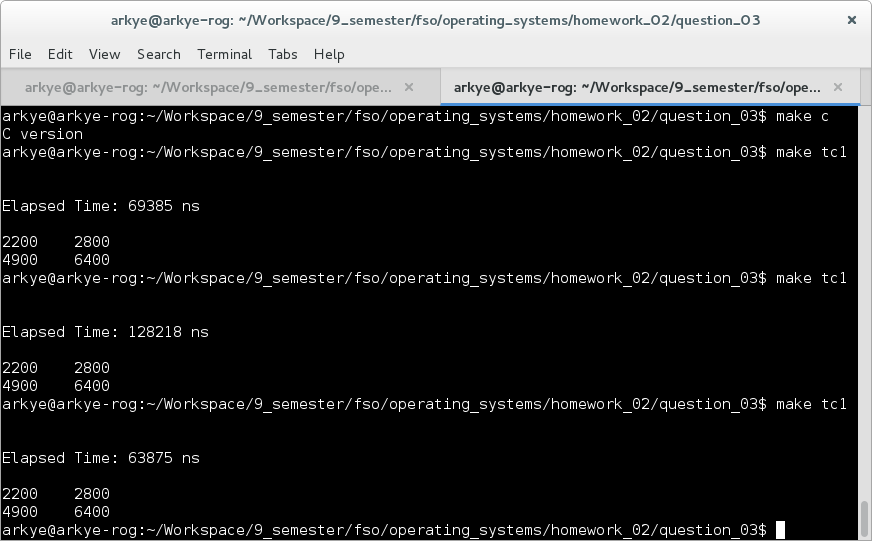
\includegraphics[scale=0.4]{c_tc1}
		\caption{Resultados da versão \texttt{q03c} com o caso de teste \texttt{tc1}.}
		\label{fig:c_tc1}
	\end{center}
\end{figure}

\begin{figure}[H]
	\begin{center}
		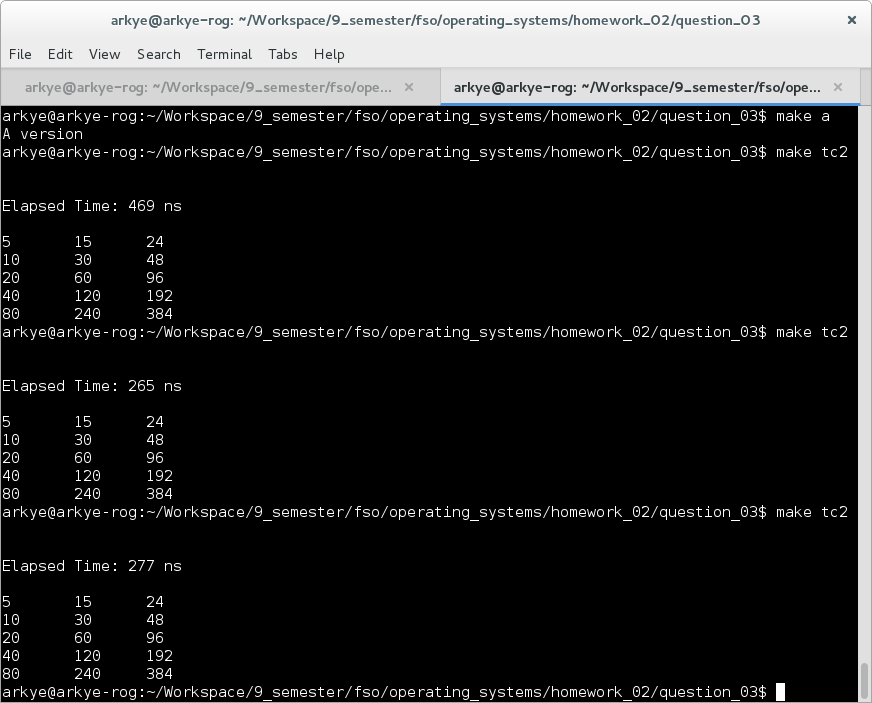
\includegraphics[scale=0.31]{a_tc2}
		\caption{Resultados da versão \texttt{q03a} com o caso de teste \texttt{tc2}.}
		\label{fig:a_tc2}
	\end{center}
\end{figure}

\begin{figure}[H]
	\begin{center}
		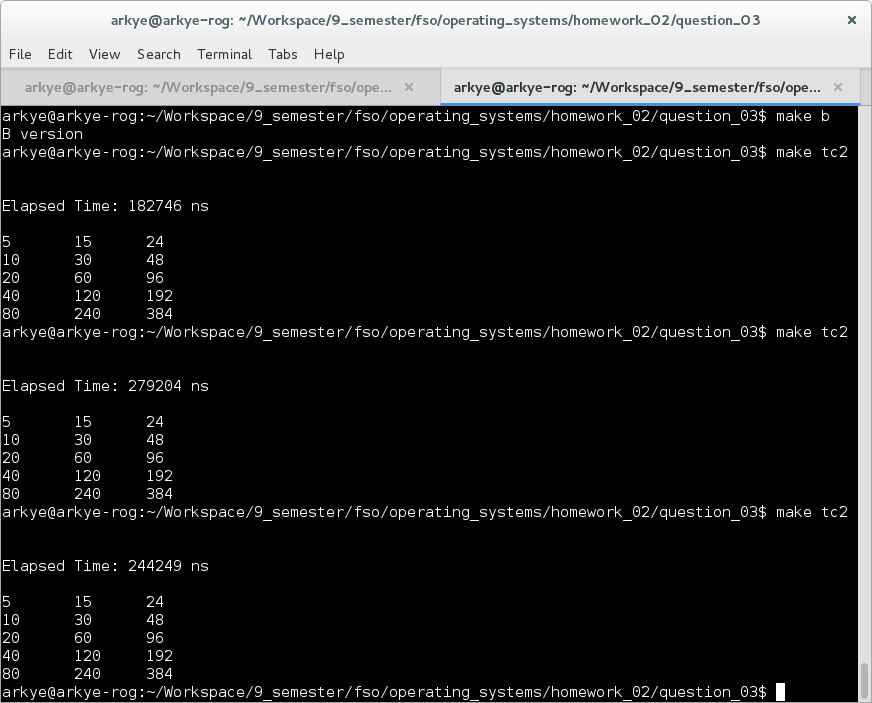
\includegraphics[scale=0.31]{b_tc2}
		\caption{Resultados da versão \texttt{q03b} com o caso de teste \texttt{tc2}.}
		\label{fig:b_tc2}
	\end{center}
\end{figure}

\begin{figure}[H]
	\begin{center}
		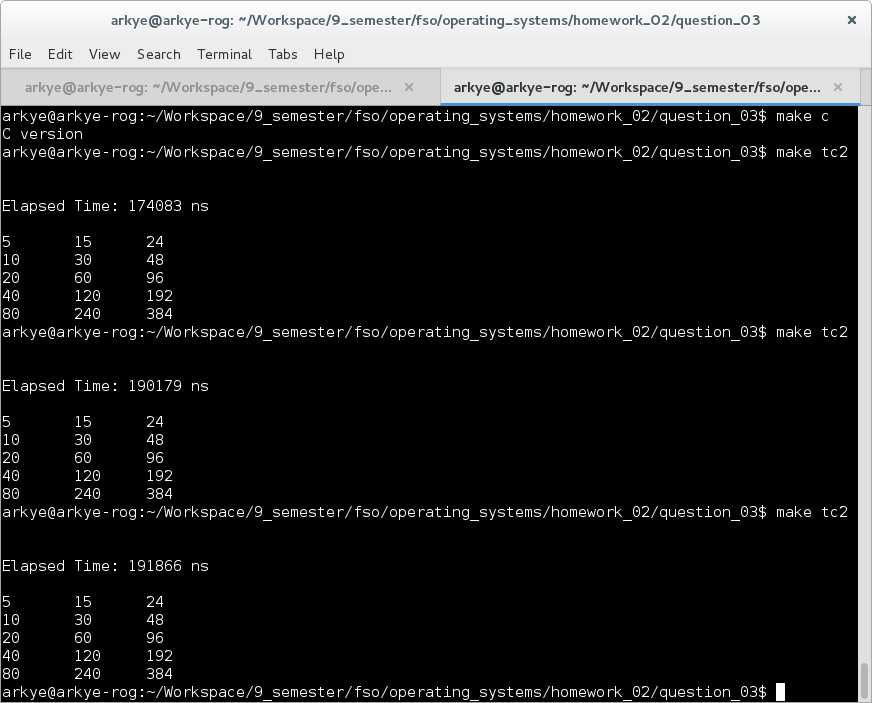
\includegraphics[scale=0.31]{c_tc2}
		\caption{Resultados da versão \texttt{q03c} com o caso de teste \texttt{tc2}.}
		\label{fig:c_tc2}
	\end{center}
\end{figure}

\begin{figure}[H]
	\begin{center}
		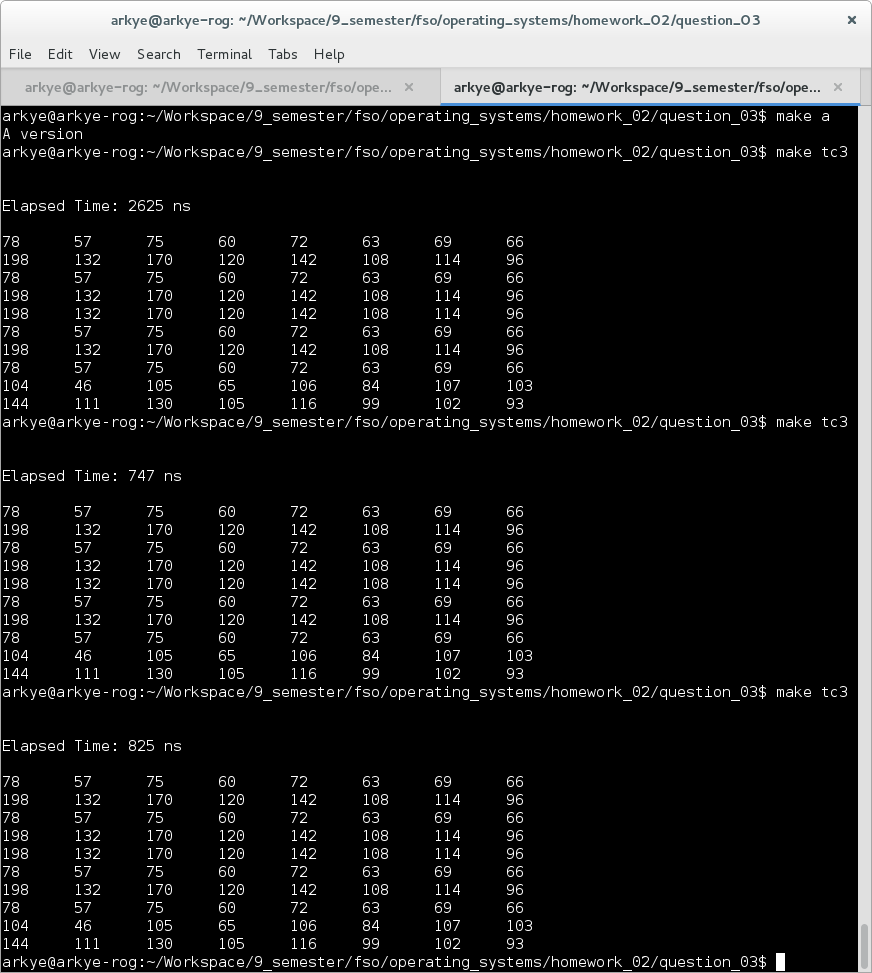
\includegraphics[scale=0.4]{a_tc3}
		\caption{Resultados da versão \texttt{q03a} com o caso de teste \texttt{tc3}.}
		\label{fig:a_tc3}
	\end{center}
\end{figure}

\begin{figure}[H]
	\begin{center}
		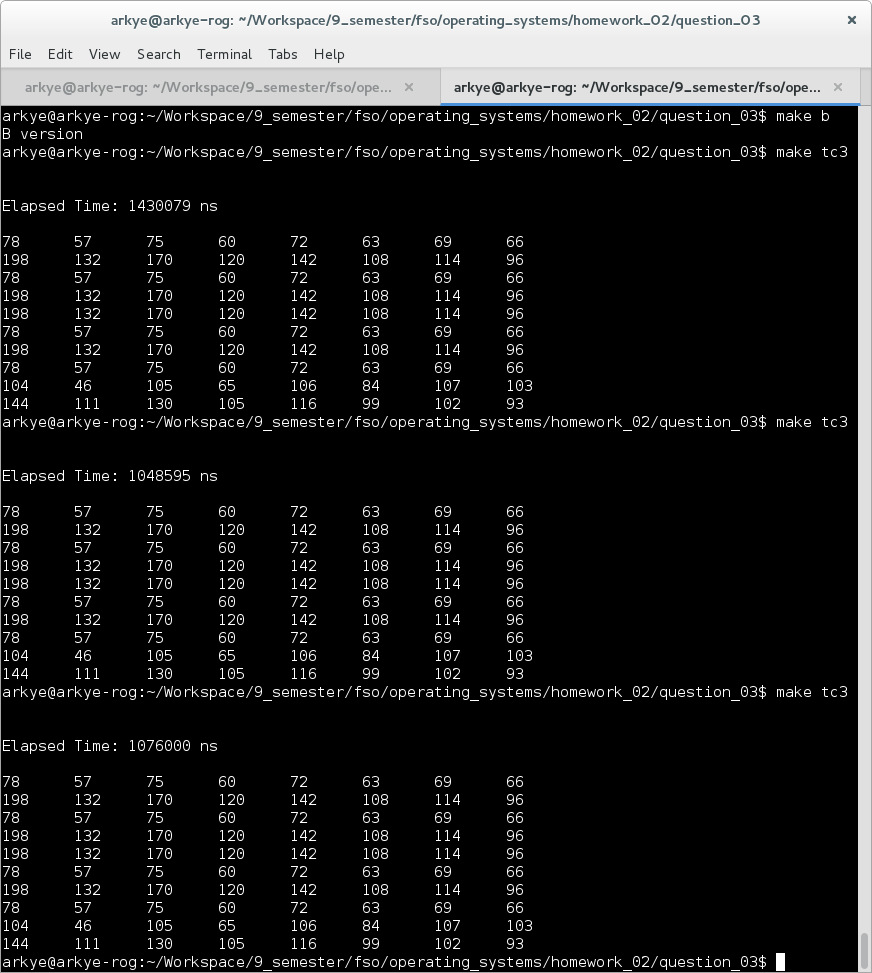
\includegraphics[scale=0.4]{b_tc3}
		\caption{Resultados da versão \texttt{q03b} com o caso de teste \texttt{tc3}.}
		\label{fig:b_tc3}
	\end{center}
\end{figure}

\begin{figure}[H]
	\begin{center}
		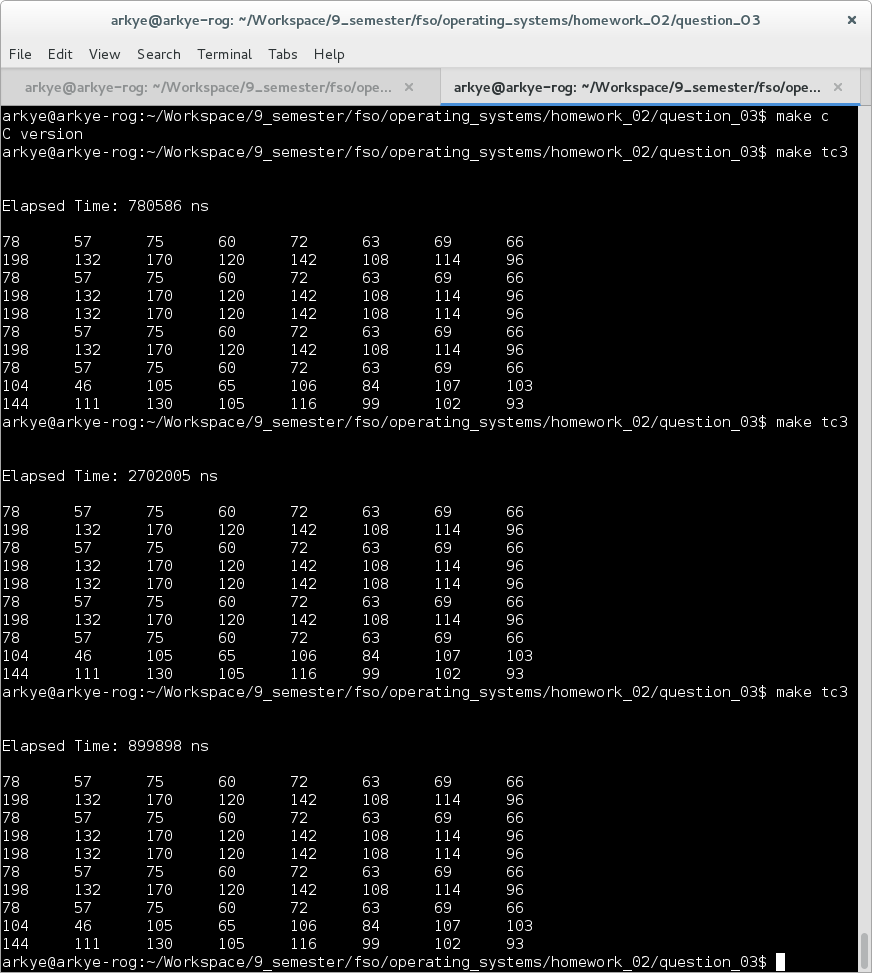
\includegraphics[scale=0.4]{c_tc3}
		\caption{Resultados da versão \texttt{q03c} com o caso de teste \texttt{tc3}.}
		\label{fig:c_tc3}
	\end{center}
\end{figure}
